\documentclass[border=10pt]{standalone} 
\usepackage[utf8]{inputenc}
\usepackage{nacal}
\usepackage{pgfplots}
\usepackage{tikz-3dplot}
\usepackage{tikz} 
\usetikzlibrary{matrix,decorations.pathreplacing}
\usetikzlibrary{calc,angles,positioning,intersections,quotes,decorations.markings}
\usepackage{tkz-euclide}

\pgfplotsset{width=10cm,height=6cm}

\begin{document}
  \def\Rojo{red!50!black}
  \def\RojoOscuro{red!20!black}
  \def\RojoClaro{red!90!black}
  \def\Verde{green!50!black}
  \def\VerdeOscuro{green!30!black}
  \def\VerdeClaro{green!50!gray}
  \def\Azul{blue!50!black}
  \def\AzulOscuro{blue!35!black}
  \def\AzulClaro{blue!60!gray}

  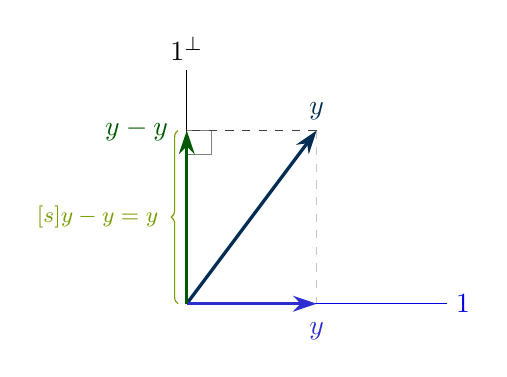
\begin{tikzpicture}[scale=1.1]
    % vértices del triángulo
    \coordinate (v1) at (0,0);
    \coordinate (v2) at (3,0); % punta eje horizontal
    \coordinate (v3) at (1.5,2);
    
    \coordinate (v4) at (1.5,0);  
    
    \coordinate (v6) at (0,2); % vector e
    \coordinate (v7) at (0,2.7); % punta eje vertical

    \tkzMarkRightAngle[size=.28,gray,very thin](v1,v6,v3) 
    
    % division del triangulo
    \draw[-,gray!45,dashed,very thin]  (v3) -- (v4);
    \draw[-,gray!50!black,dashed,very thin]  (v3) -- (v6);

    % triangulo
    \draw[color=blue!90!black,very thin]  (v1) -- (v2) node [right]  {$\Span{\Vect{1}}$};
    \draw[very thin]  (v1) -- (v7) node [above]  {$\Span{\Vect{1}}^\perp$};
    \draw[-{Stealth[length=3mm, width=2mm]},very thick,green!35!blue!50!black] (v1) -- (v3) node [above]  {$\Vect{y}$};
    
    \draw[-{Stealth[length=3mm, width=2mm]},very thick,blue!65!gray] (v1) -- (v4) node [below,yshift=-1mm]  {$\Vect{\Media{y}}$};
    \draw[-{Stealth[length=3mm, width=2mm]},very thick,green!35!black] (v1) -- (v6) node [left,xshift=-1mm]   {$\Vect{y}-\Vect{\Media{y}}$};

    % CORRECCIÓN: Trazamos de arriba a abajo usando mirror. Evita el conflicto con tkz-euclide.
    \draw[decorate, decoration={brace,mirror},green!45!orange!85!black] (-0.1,2) -- (-0.1,0) node [midway, anchor=east, xshift=-1mm, outer sep=1pt, font=\footnotesize]{${\norma[s]{\Vect{y}-\Vect{\Media{y}}}}=\dt{\Vect{y}}$};
    % gray!85!black
  \end{tikzpicture} 
\end{document}
